% CVPR 2025 Paper Template; see https://github.com/cvpr-org/author-kit

\documentclass[10pt,twocolumn,letterpaper]{article}

\usepackage[T5]{fontenc} % Encoding for Vietnamese
\usepackage[utf8]{inputenc} % Allow UTF-8 input
\usepackage[vietnam]{babel} % Vietnamese language support
\usepackage{float}
\usepackage{amsmath}        % Hỗ trợ toán học
\usepackage{amssymb}        % Ký hiệu toán học
\usepackage{amsfonts}       % Font chữ toán học
\usepackage{mdframed}       % Tạo khung

%%%%%%%%% PAPER TYPE  - PLEASE UPDATE FOR FINAL VERSION
% \usepackage{cvpr}              % To produce the CAMERA-READY version
\usepackage{cvpr}      % To produce the REVIEW version
% \usepackage[pagenumbers]{cvpr} % To force page numbers, e.g. for an arXiv version

% Import additional packages in the preamble file, before hyperref
%
% --- inline annotations
%
\newcommand{\red}[1]{{\color{red}#1}}
\newcommand{\todo}[1]{{\color{red}#1}}
\newcommand{\TODO}[1]{\textbf{\color{red}[TODO: #1]}}
% --- disable by uncommenting  
% \renewcommand{\TODO}[1]{}
% \renewcommand{\todo}[1]{#1}



% It is strongly recommended to use hyperref, especially for the review version.
% hyperref with option pagebackref eases the reviewers' job.
% Please disable hyperref *only* if you encounter grave issues, 
% e.g. with the file validation for the camera-ready version.
%
% If you comment hyperref and then uncomment it, you should delete *.aux before re-running LaTeX.
% (Or just hit 'q' on the first LaTeX run, let it finish, and you should be clear).
\definecolor{cvprblue}{rgb}{0.21,0.49,0.74}
\usepackage[pagebackref,breaklinks,colorlinks,allcolors=cvprblue]{hyperref}

%%%%%%%%% PAPER ID  - PLEASE UPDATE
\def\paperID{*****} % *** Enter the Paper ID here
\def\confName{CS115}
\def\confYear{2024}

%%%%%%%%% TITLE - PLEASE UPDATE
\title{Variational Autoencoder (VAE)}

%%%%%%%%% AUTHORS - PLEASE UPDATE
\author{
    Thanh Bui Ngoc Thien \\
    University of Information Technology - VNU \\
    {\tt\small 23521436@gm.uit.edu.vn}
    \and
    Nam Nguyen Pham Phuong \\
    University of Information Technology - VNU \\
    {\tt\small 23520978@gm.uit.edu.vn}
    \and
    Cuong Dang Quoc \\
    University of Information Technology - VNU \\
    {\tt\small 23520192@gm.uit.edu.vn}
}


\begin{document}
\maketitle
\begin{abstract}
Variational Autoencoders (VAEs) are a powerful probabilistic framework that bridges mathematical modeling and deep learning. This paper delves into the mathematical foundations of VAEs, with a focus on deriving the Evidence Lower Bound (ELBO) as a core optimization objective. Key mathematical constructs such as the Kullback-Leibler divergence and the reparameterization trick are analyzed, enabling efficient gradient computation and stable training. Additionally, we provide rigorous insights into how latent space modeling with Gaussian distributions supports data generation and reconstruction tasks. The study highlights the interplay between mathematical rigor and computational efficiency, making VAEs an essential tool in dimensionality reduction, anomaly detection, and generative modeling. This work aims to deepen the understanding of VAEs' mathematical principles, offering a strong foundation for further exploration in both academic and applied contexts.
\end{abstract}    
\section{Introduction}
\label{sec:intro}

\subsection{Basic Structure of VAE}

VAE consists of three main components: the encoder, the latent space, and the decoder ~\cite{chan2025tutorial}.

\begin{itemize}
    \item \textbf{Encoder:}
    The encoder takes input data and transforms it into a representation within the \textit{latent space}. Unlike traditional AE, the encoder in VAE learns a probabilistic distribution instead of fixed points, allowing for more flexible and uncertainty-aware data representation.

    \item \textbf{Latent Space:}  
    The latent space in VAE is a continuous and well-organized space. Each point in this space represents a latent state of the data. The continuity and smoothness of the latent space allow the model to generate new data by sampling points from it.

    \item \textbf{Decoder:}  
    The decoder receives information from the latent space and reconstructs the original data. Additionally, it can generate new data by sampling points from the latent space, making VAE a highly effective generative model.
\end{itemize}

The key strength of VAE lies in its ability to balance accurate data reconstruction with the organization of the latent space, facilitating meaningful data generation.

\begin{figure}[H]
    \centering
    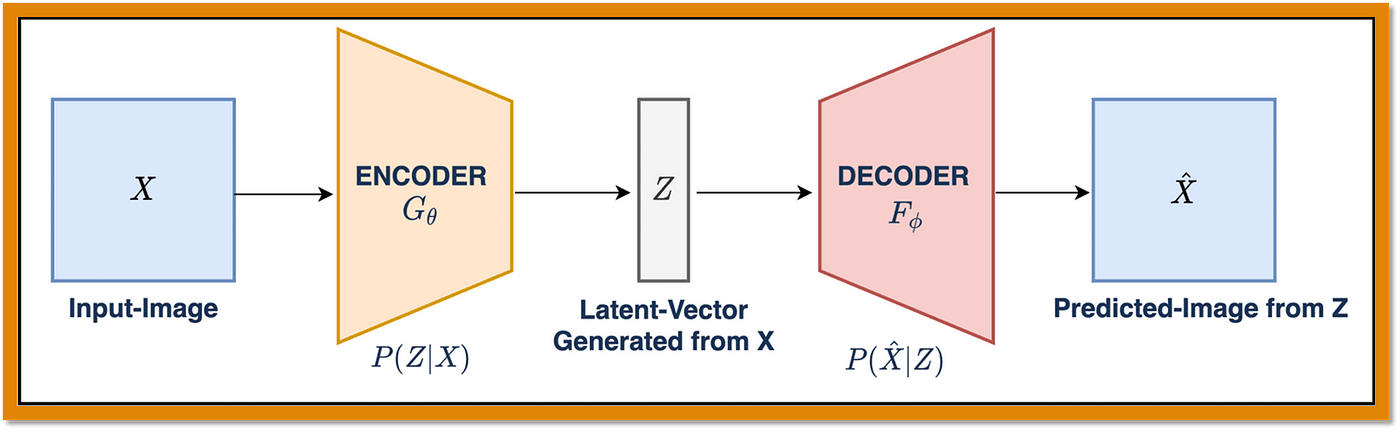
\includegraphics[width=1.0\linewidth]{sec/VAE.png}
    \caption{VAE Structure}
\end{figure}

\subsection{Why Choose VAE}

While the traditional Autoencoder excels at compressing and reconstructing data, it has limitations that VAE addresses. Here are the main reasons why VAE is preferred:

\begin{itemize}
    \item \textbf{Data Generation:}  
    Traditional AE only reconstructs learned data, whereas VAE can generate new data by sampling from the latent space.

    \item \textbf{Smooth Latent Space:}  
    The latent space of VAE is continuous and smooth, ensuring that generated samples are reasonable even when sampled randomly.

    \item \textbf{Better Generalization:}  
    VAE utilizes regularization techniques to avoid overfitting and improve its generalization capabilities on unseen data.

    \item \textbf{Uncertainty Handling:}  
    VAE can learn and represent uncertainty in the data, a capability absent in traditional AE.
\end{itemize}

Thanks to these advantages, VAE serves as a powerful tool for data compression, reconstruction, and diverse applications such as image synthesis, anomaly detection, and data augmentation.
\section{Some mathematical symbols are used}
\begin{itemize}
    \item $p(\mathbf{x})$: The true distribution of $\mathbf{x}$. It is never known. The whole universe of diffusion models is to find ways to draw samples from $p(\mathbf{x})$. If we knew $p(\mathbf{x})$ (say, we have a formula that describes $p(\mathbf{x})$), we can just draw a sample $\mathbf{x}$ that maximizes $\log p(\mathbf{x})$.
    
    \item $p(z)$: The distribution of the latent variable. Typically, we make it a zero-mean unit-variance Gaussian $\mathcal{N}(0, \mathbf{I})$. One reason is that linear transformation of a Gaussian remains a Gaussian, and so this makes the data processing easier. It was mentioned that any distribution can be generated by mapping a Gaussian through a sufficiently complicated function.
    
    \item $p(z|\mathbf{x})$: The conditional distribution associated with the \textit{encoder}, which tells us the likelihood of $z$ when given $\mathbf{x}$. We have no access to it. $p(z|\mathbf{x})$ itself is not the encoder, but the encoder has to do something so that it will behave consistently with $p(z|\mathbf{x})$.
    
    \item $p(\mathbf{x}|z)$: The conditional distribution associated with the \textit{decoder}, which tells us the posterior probability of getting $\mathbf{x}$ given $z$. Again, we have no access to it.
\end{itemize}

\vspace{10pt}
In reality, $p(z|\mathbf{x})$ and $p(\mathbf{x}|z)$ are very difficult to calculate as well as their complications. Thus, we suggest using two proxy distributions:
\begin{itemize}
    \item $q_{\phi}(z|\mathbf{x})$: The proxy for $p(z|\mathbf{x})$, which is also the distribution associated with the \textit{encoder} ~\cite{james1980monte}. 
    $q_{\phi}(z|\mathbf{x})$ can be any directed graphical model and it can be parameterized using deep neural networks. For example, we can define
    \[
    (\mu, \sigma^2) = \text{EncoderNetwork}_{\phi}(\mathbf{x}),
    \]
    \[
    q_{\phi}(z|\mathbf{x}) = \mathcal{N}(z \mid \mu, \text{diag}(\sigma^2)).
    \]
    This model is widely used because of its tractability and computational efficiency.
    
    \item $p_{\theta}(\mathbf{x}|z)$: The proxy for $p(\mathbf{x}|z)$, which is also the distribution associated with the \textit{decoder}. 
    Like the encoder, the decoder can be parameterized by a deep neural network. For example, we can define
    \[
    f_{\theta}(z) = \text{DecoderNetwork}_{\theta}(z),
    \]
    \[
    p_{\theta}(\mathbf{x}|z) = \mathcal{N}(\mathbf{x} \mid f_{\theta}(z), \sigma_{\text{dec}}^2 \mathbf{I}),
    \]
    where $\sigma_{\text{dec}}$ is a hyperparameter that can be pre-determined or it can be learned.
\end{itemize}
The relationship between the input $\mathbf{x}$ and the latent $z$, as well as the conditional distributions, are summarized below.
\begin{figure}[H]
    \centering
    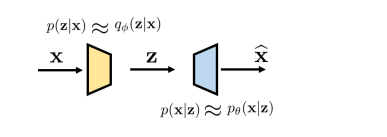
\includegraphics[width=1.25\linewidth]{sec/VAE_relation.png}
    \caption{In a variational autoencoder, the variables $\mathbf{x}$ and $z$ are connected by the conditional distributions $p(z|\mathbf{x})$ and $p(\mathbf{x}|z)$.}
\end{figure}

\section{Build Encoder and Decoder in Variational AutoEncoder}

Suppose that we have a random variable $x \in \mathbb{R}^d$ and a latent variable $z \in \mathbb{R}^d$ such that ~\cite{cemgil2020autoencoding}:
\[
x \sim p(x) = \mathcal{N}(x \mid \mu, \sigma^2 \mathbf{I}),
\]
\[
z \sim p(z) = \mathcal{N}(z \mid 0, \mathbf{I}).
\]
We want to construct a Variational Autoencoder. By this, we mean that we want to build two mappings $\text{Encoder}(\cdot)$ and $\text{Decoder}(\cdot)$. The encoder will take a sample $x$ and map it to the latent variable $z$, whereas the decoder will take the latent variable $z$ and map it to the generated variable $\hat{x}$. 

If we knew what $p(x)$ is, then there is a trivial solution where:
\[
z = \frac{x - \mu}{\sigma}, \quad \hat{x} = \mu + \sigma z.
\]

In this case, the true distributions can be determined and expressed in terms of delta functions:
\[
p(x \mid z) = \delta \big(x - (\sigma z + \mu)\big),
\]
\[
p(z \mid x) = \delta \big(z - \frac{x - \mu}{\sigma}\big).
\]

\subsection{Definition of Dirac Delta Function}
\begin{itemize}
    \item The Dirac delta function  ~\cite{wheeler1997dirac} as the limit when $a \to 0$ of a sequence of normalized Gaussian distributions centered at 0 is expressed as:
    \[
    \delta_a(x) = \frac{1}{|a| \sqrt{\pi}} e^{-\left(\frac{x}{a}\right)^2}.
    \]
    \item Where:
    \begin{itemize}
        \item $a$ is the scaling parameter,
        \item $|a|$ is the absolute value of $a$,
        \item $\sqrt{\pi}$ is the normalization constant,
        \item $e^{-\left(\frac{x}{a}\right)^2}$ is the Gaussian exponential function.
    \end{itemize}
\end{itemize}

\begin{figure}[H]
    \centering
    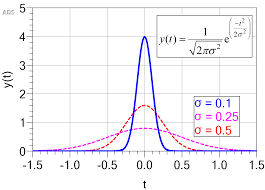
\includegraphics[width=1\linewidth]{sec/dirac.png}
    \caption{Dirac Delta Function}
\end{figure}


\subsection{Encoder and Decoder Construction}
Suppose now that we do not know $p(x)$, so we need to build an encoder and a decoder to estimate $z$ and $\hat{x}$.

\textbf{Encoder Design:}
The encoder takes the input $x$ and generates a pair of parameters $\hat{\mu}(x)$ and $\hat{\sigma}^2(x)$, denoting the parameters of a Gaussian ~\cite{zhang2015kl}. Then, we define $q_\phi(z \mid x)$ as:
\[
(\hat{\mu}(x), \hat{\sigma}^2(x)) = \text{Encoder}_\phi(x),
\]
\[
q_\phi(z \mid x) = \mathcal{N}(z \mid \hat{\mu}(x), \hat{\sigma}^2(x)\mathbf{I}).
\]

For simplicity:
\[
\hat{\mu}(x) = ax + b, \quad \hat{\sigma}^2(x) = t^2,
\]
where $a$, $b$, and $t$ are learned parameters. Substituting, we get:
\[
q_\phi(z \mid x) = \mathcal{N}(z \mid ax + b, t^2 \mathbf{I}).
\]

\textbf{Decoder Design:}
The decoder takes $z$ and reconstructs $x$ using:
\[
(\mu_e(z), \sigma_e^2(z)) = \text{Decoder}_\theta(z),
\]
\[
p_\theta(x \mid z) = \mathcal{N}(x \mid \mu_e(z), \sigma_e^2(z)\mathbf{I}).
\]

Similarly, for simplicity:
\[
\mu_e(z) = cz + v, \quad \sigma_e^2(z) = s^2,
\]
where $c$, $v$, and $s$ are learned parameters. Substituting, we get:
\[
p_\theta(x \mid z) = \mathcal{N}(x \mid cz + v, s^2 \mathbf{I}).
\]

\section{Evidence Lower Bound}

If we treat ${\phi}$ and ${\theta}$ as two optimization variables, we need an objective function (Loss function) to optimize these two parameters. The Loss function we use here is called Evidence Lower Bound (ELBO).

\subsection*{Definition (Evidence Lower Bound):}
\begin{equation}
\text{ELBO}(x) = \mathbb{E}_{q_\phi(z|x)} \left[ \log \frac{p(x, z)}{q_\phi(z|x)} \right].
\end{equation}

As mentioned earlier, \(p(x)\) is the marginal probability of the observation variable \(x\), calculated as:
\[
p(x) = \int p(x, z) \, dz = \int p(x \mid z) p(z) \, dz.
\]

\begin{itemize}
    \item We need to optimize this probability to motivate the model to achieve the best data distribution, thereby simulating and understanding the data. However, calculating this integral is very complicated due to the large space of \(z\) and the lack of a closed-form solution for \(p(x \mid z)\) and \(p(z)\).
    \item To address this, we build the relationship between \(p(x)\) and \(\text{ELBO}(x)\). We suggest the following theorem:
\end{itemize}

\subsection*{Theorem 1.1. Decomposition of Log-Likelihood:}
The log-likelihood \(\log p(x)\) can be decomposed as:
\[
\log p(x) = \mathbb{E}_{q_\phi(z|x)} \left[ \log \frac{p(x, z)}{q_\phi(z|x)} \right] + D_{\mathrm{KL}}(q_\phi(z|x) \| p(z|x)).
\]

\subsection*{Proof:}
Using \(q_\phi(z|x)\) as a proxy for \(p(x)\), we have:
\[
\log p(x) = \log p(x) \times \underbrace{\int q_\phi(z|x) dz}_{=1}.
\]

This implies:
\[
\log p(x) = \mathbb{E}_{q_\phi(z|x)} [\log p(x)].
\]

We define the Kullback-Leibler Divergence ~\cite{shlens2014kl} between two continuous distributions as:
\[
D_{\text{KL}}(P \,\|\, Q) = \int_{-\infty}^\infty p(x) \log \left( \frac{p(x)}{q(x)} \right) \, dx = \mathbb{E}_{p(x)} \left[\log \frac{p(x)}{q(x)} \right].
\]

\begin{figure}[H]
    \centering
    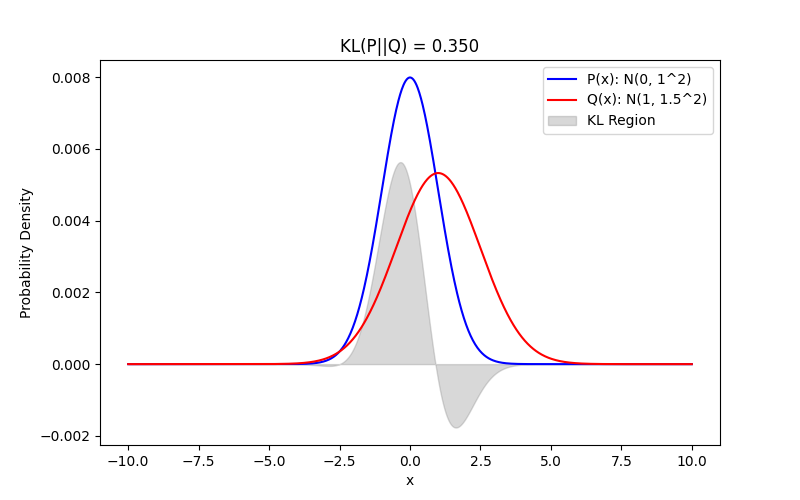
\includegraphics[width=1\linewidth]{sec/KL.png}
    \caption{Kullback-Leibler Divergence}
\end{figure}

Using Bayes' theorem (\(p(x, z) = p(z|x)p(x)\)) ~\cite{dosovitskiy2021imageworth16x16words}:
\[
\mathbb{E}_{q_\phi(z|x)}[\log p(x)] = \mathbb{E}_{q_\phi(z|x)} \left[\log \frac{p(x, z)}{p(z|x)}\right].
\]

Rewriting:
\begin{align}
\mathbb{E}_{q_\phi(z|x)} [\log p(x)] &= \mathbb{E}_{q_\phi(z|x)} 
\Big[ \log \frac{p(x, z)}{q_\phi(z|x)} \Big] \nonumber \\
&\quad + \mathbb{E}_{q_\phi(z|x)} 
\Big[ \log \frac{q_\phi(z|x)}{p(z|x)} \Big].
\end{align}


This simplifies to:
\[
\log p(x) = \text{ELBO}(x) + D_{\mathrm{KL}}(q_\phi(z|x) \| p(z|x)).
\]

\subsection*{Theorem 1.2. ELBO Decomposition:}
The ELBO can be expressed as:
\begin{equation}
\text{ELBO}(x) = \mathbb{E}_{q_\phi(z|x)} 
\big[\log p_\theta(x|z)\big] 
- D_{\text{KL}}(q_\phi(z|x) \| p(z)).
\end{equation}

\subsection*{Proof:}
Breaking the ELBO into two terms:
\begin{align*}
\text{ELBO}(x) &\overset{\text{def}}{=} \mathbb{E}_{q_\phi(z|x)} \big[ \log \frac{p(x, z)}{q_\phi(z|x)} \big] \\
&= \mathbb{E}_{q_\phi(z|x)} \big[ \log \frac{p(x|z)p(z)}{q_\phi(z|x)} \big] \\
&= \mathbb{E}_{q_\phi(z|x)} \big[ \log p(x|z) \big] + \mathbb{E}_{q_\phi(z|x)} \big[ \log \frac{p(z)}{q_\phi(z|x)} \big] \\
&= \mathbb{E}_{q_\phi(z|x)} \big[ \log p_\theta(x|z) \big] - D_{\text{KL}} \big( q_\phi(z|x) \| p(z) \big).
\end{align*}

\subsection*{ELBO Terms:}
\begin{itemize}
    \item \textbf{Reconstruction:} The first term, \(\mathbb{E}_{q_\phi(z|x)} [\log p_\theta(x|z)]\), measures the decoder's ability to reconstruct \(x\) from \(z\). This term is maximized when the decoder is accurate.
    \item \textbf{Prior Matching:} The second term, \(D_{\text{KL}}(q_\phi(z|x) \| p(z))\), regularizes \(q_\phi(z|x)\) to align with the prior \(p(z)\), typically \(\mathcal{N}(0, I)\).
\end{itemize}

\section{Optimization in VAE}

\subsection{Objective Function}
The optimization objective of the VAE is to maximize the Evidence Lower Bound (ELBO):
\begin{equation}
(\phi, \theta) = \arg\max_{\phi, \theta} \sum_{x \in \mathcal{X}} \text{ELBO}(x),
\end{equation}
where \(\mathcal{X} = \{x^{(\ell)} \mid \ell = 1, \dots, L\}\) is the training dataset.

The main challenge in optimizing the VAE lies in the intractability of the ELBO gradient with respect to \((\phi, \theta)\). Since modern neural network optimizers rely on first-order methods like gradient descent and backpropagation, this intractability makes training difficult.

\subsection{Gradient Computation for ELBO}
The gradient of the ELBO can be expressed as:
\begin{align}
\nabla_{\theta, \phi} \text{ELBO}(x) &= \nabla_{\theta, \phi} 
\mathbb{E}_{q_\phi(z|x)} 
\left[
\log \frac{p_\theta(x, z)}{q_\phi(z|x)}
\right] \nonumber \\
&= \nabla_{\theta, \phi} 
\mathbb{E}_{q_\phi(z|x)} 
\left[
\log p_\theta(x, z) - \log q_\phi(z|x)
\right].
\end{align}

---

\subsubsection*{Gradient with Respect to \(\theta\)}
The gradient with respect to \(\theta\) can be derived as:
\begin{align}
\nabla_\theta \text{ELBO}(x) &= \mathbb{E}_{q_\phi(z|x)}
\left[
\nabla_\theta \log p_\theta(x, z)
\right].
\end{align}

Using Monte Carlo approximation, we obtain:
\begin{equation}
\nabla_\theta \text{ELBO}(x) \approx 
\frac{1}{L} \sum_{\ell=1}^L 
\nabla_\theta \log p_\theta(x, z^{(\ell)}),
\end{equation}
where \(z^{(\ell)} \sim q_\phi(z|x)\).

---

\subsubsection*{Gradient with Respect to \(\phi\)}
The gradient with respect to \(\phi\) is more challenging:
\begin{align}
\nabla_\phi \text{ELBO}(x) &= \mathbb{E}_{q_\phi(z|x)} 
\left[
\nabla_\phi \log p_\theta(x, z) - \nabla_\phi \log q_\phi(z|x)
\right].
\end{align}

Using Monte Carlo approximation for the second term:
\begin{equation}
\nabla_\phi \text{ELBO}(x) \approx \frac{1}{L} \sum_{\ell=1}^L 
\nabla_\phi 
\left(
- \log q_\phi(z^{(\ell)}|x)
\right),
\end{equation}
where \(z^{(\ell)} \sim q_\phi(z|x)\).

---

\subsection{Reparameterization Trick}
To simplify gradient computation, the \textbf{Reparameterization Trick} is introduced. Recall that the latent variable \(z\) is a sample drawn from \(q_\phi(z|x)\). The reparameterization trick expresses \(z\) as a differentiable and invertible transformation of another random variable \(\epsilon\), independent of \(x\) and \(\phi\).

Suppose:
\begin{equation}
z \sim q_\phi(z|x) = \mathcal{N}(z \mid \mu, \text{diag}(\sigma^2)),
\end{equation}
we define:
\begin{equation}
z = g(\epsilon, \phi, x) = \epsilon \odot \sigma + \mu, \quad \epsilon \sim \mathcal{N}(0, I),
\end{equation}
where \(\odot\) denotes elementwise multiplication, and \(\phi = (\mu, \sigma^2)\).

---

\subsubsection*{Jacobian Simplification}
$\frac{\partial z}{\partial \epsilon}$ is the Jacobian, we can define that:
\[
\frac{\partial z}{\partial \epsilon} =
\begin{bmatrix}
\frac{\partial z_1}{\partial \epsilon_1} & \frac{\partial z_1}{\partial \epsilon_2} & \cdots & \frac{\partial z_1}{\partial \epsilon_d} \\
\frac{\partial z_2}{\partial \epsilon_1} & \frac{\partial z_2}{\partial \epsilon_2} & \cdots & \frac{\partial z_2}{\partial \epsilon_d} \\
\vdots & \vdots & \ddots & \vdots \\
\frac{\partial z_d}{\partial \epsilon_1} & \frac{\partial z_d}{\partial \epsilon_2} & \cdots & \frac{\partial z_d}{\partial \epsilon_d}
\end{bmatrix}.
\]
The expression for each component $i$ is:
\[
z_i = \sigma_i \epsilon_i + \mu_i
\]

---

\subsection{Gradient Computation with Reparameterization}
Using the reparameterization trick, we aim to compute:
\[
\nabla_\phi \mathbb{E}_{q_\phi(z|x)}[f(z)] = \mathbb{E}_{p(\epsilon)}[\nabla_\phi f(z)],
\]
where \(f(z)\) is some function of \(z\) (e.g., \(f(z) = -\log q_\phi(z|x)\)).

Substituting \(f(z) = -\log q_\phi(z|x)\), we obtain:
\[
\nabla_\phi \mathbb{E}_{q_\phi(z|x)}[-\log q_\phi(z|x)] \approx \frac{1}{L} \sum_{\ell=1}^L \nabla_\phi \log \det \left( \frac{\partial z^{(\ell)}}{\partial \epsilon^{(\ell)}} \right),
\]
where \(z^{(\ell)} = g(\epsilon^{(\ell)}, \phi, x)\).

---

\subsection{Monte Carlo Approximation}
Using Monte Carlo ~\cite{james1980monte, kroese2014monte}, the expectation can be approximated as:
\[
\mathbb{E}_{q_\phi(z|x)}[f(z)] \approx \frac{1}{L} \sum_{\ell=1}^L f(z^{(\ell)}),
\]
where \(z^{(\ell)} = g(\epsilon^{(\ell)}, \phi, x)\) and \(\epsilon^{(\ell)} \sim \mathcal{N}(0, I)\).

This reparameterization allows gradients to flow through \(\phi = (\mu, \sigma^2)\) efficiently.



\section{Specific Structure of VAE}

\subsection{Encoder}

\[
(\mu, \sigma^2) = \text{EncoderNetwork}_\phi(x)
\]
\[
q_\phi(z|x) = \mathcal{N}(z | \mu, \sigma^2 I)
\]

The parameters \( \mu \) and \( \sigma \) are technically neural networks because they are outputs of \( \text{EncoderNetwork}_\phi(\cdot) \).

\vspace{0.3cm}

We denote them as:
\[
\mu = \mu_\phi(x) \quad \text{and} \quad \sigma^2 = \sigma^2_\phi(x).
\]

Given the \(\ell\)-th training sample \( x^{(\ell)} \), the latent variable \( z^{(\ell)} \) is sampled as:
\[
z^{(\ell)} \sim \mathcal{N} \left( z \mid \mu_\phi(x^{(\ell)}), \sigma^2_\phi(x^{(\ell)})I \right).
\]

\subsection{Sampling with Reparameterization Trick}

From the Gaussian, we draw a sample \( z^{(\ell)} \):
\[
z^{(\ell)} = \mu_\phi(x^{(\ell)}) + \sigma_\phi(x^{(\ell)}) \epsilon, \quad \epsilon \sim \mathcal{N}(0, \textbf{I}).
\]
\begin{figure}
    \centering
    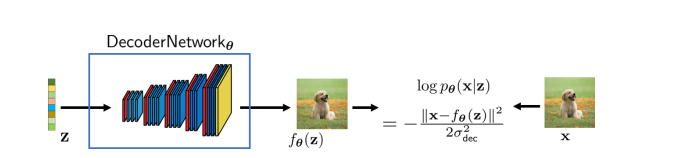
\includegraphics[width=1\linewidth]{sec/anh02.png}
    \caption{Implementation of a VAE encoder. The neural network takes \( x \) and estimates \( \mu_\phi \) and \( \sigma^2_\phi \).}
    \label{fig:vae_encoder}
\end{figure}

\subsection{KL Divergence of Two Gaussians}
\begin{mdframed}
\textbf{Theorem 1.3: KL-Divergence of Two Gaussians} ~\cite{chan2025tutorial}

The KL divergence for two \(d\)-dimensional Gaussian distributions \( \mathcal{N}(\mu_0, \Sigma_0) \) and \( \mathcal{N}(\mu_1, \Sigma_1) \) is:
\begin{align*}
D_{\text{KL}}\left(\mathcal{N}(\mu_0, \Sigma_0) \parallel \mathcal{N}(\mu_1, \Sigma_1)\right) 
&= \frac{1}{2} \Big[ \text{Tr}(\Sigma_1^{-1} \Sigma_0) - d \\
&\quad + (\mu_1 - \mu_0)^T \Sigma_1^{-1} (\mu_1 - \mu_0) \\
&\quad + \log \frac{\det \Sigma_1}{\det \Sigma_0} \Big].
\end{align*}
\end{mdframed}

\subsection{KL Divergence in VAE}

\textbf{Substituting Specific Distributions:}
\[
\mu_0 = \mu_\phi(x), \quad \Sigma_0 = \sigma_\phi^2(x) \textbf{I}, \quad \mu_1 = 0, \quad \Sigma_1 = \textbf{I}.
\]

\textbf{Simplified KL Divergence:}
\[
D_{\text{KL}}\left(q_\phi(z \mid x) \parallel p(z)\right) = 
\frac{1}{2} \Big[ 
\sigma_\phi^2(x) d - d + \|\mu_\phi(x)\|^2 - 2 \log \sigma_\phi(x) 
\Big].
\]

Here, \(d\) is the dimension of the latent vector \(z\).

\subsection{Decoder}

The decoder network, \( \text{DecoderNetwork}_\theta(\cdot) \), maps a latent variable \( z \) to a generated image or data point:
\[
f_\theta(z) = \text{DecoderNetwork}_\theta(z).
\]

The likelihood of the data given the latent variable, \( p_\theta(x \mid z) \), is assumed to follow a Gaussian distribution:
\[
p_\theta(x \mid z) = \mathcal{N}(x \mid f_\theta(z), \sigma_{\text{dec}}^2 I),
\]
where \( \sigma_{\text{dec}} \) is a hyperparameter that determines the variance of the Gaussian distribution. 

\textbf{Reparameterization Trick:} The generated data point \( \widehat{x} \) can be sampled as:
\[
\widehat{x} = f_\theta(z) + \sigma_{\text{dec}} \epsilon, \quad \epsilon \sim \mathcal{N}(0, I).
\]

\subsection*{Log-Likelihood of \( p_\theta(x \mid z) \)}

The log-likelihood of the data given \( z \) can be expressed as:
\begin{align*}
  \log p_\theta(x|z) &= \log \mathcal{N}(x \mid f_\theta(z), \sigma_{\text{dec}}^2 I) \\
  &= - \frac{\|x - f_\theta(z)\|^2}{2 \sigma_{\text{dec}}^2} 
  - \frac{d}{2} \log(2\pi \sigma_{\text{dec}}^2),
\end{align*}
where \( d \) is the dimensionality of \( x \). 

The constant term \( -\frac{d}{2} \log(2\pi \sigma_{\text{dec}}^2) \) does not depend on the model parameters \( \theta \) and can be ignored during optimization.

\vspace{10pt}
\textbf{Explanation:}
\begin{itemize}
    \item \( f_\theta(z) \): The deterministic mapping from \( z \) to the mean of the Gaussian distribution.
    \item \( \sigma_{\text{dec}}^2 \): Variance of the Gaussian distribution, controlling how tightly \( x \) is expected to cluster around \( f_\theta(z) \).
\end{itemize}


\subsection{VAE Training: Optimization Objective}

To train a VAE, we need to solve the optimization problem ~\cite{chan2025tutorial}:
\[
\arg\max_{\theta, \phi} \sum_{x \in \mathcal{X}} \text{ELBO}_{\phi, \theta}(x),
\]
where:
\[
\text{ELBO}_{\phi, \theta}(x) = \text{Reconstruction Term} + \text{KL Divergence Term}.
\]

\subsection*{Reconstruction Term}
\[
- \frac{1}{M} \sum_{m=1}^M 
\frac{\|x - f_\theta\left(\mu_\phi(x) + \sigma_\phi(x)\epsilon^{(m)}\right)\|^2}{2\sigma_\text{dec}^2}.
\]

\subsection*{KL Divergence Term}
\[
+ \frac{1}{2} \Big(\sigma_\phi^2(x)d - d + \|\mu_\phi(x)\|^2 - 2 \log \sigma_\phi(x) \Big).
\]

\subsection*{Explanation of Terms}
\begin{itemize}
    \item \( \mu_\phi(x) \): Mean output of the encoder.
    \item \( \sigma_\phi(x) \): Standard deviation output of the encoder.
    \item \( d \): Dimension of the latent variable \(z\).
\end{itemize}

\section{Applications of VAE}
\begin{itemize}
    \item Image Generation
    \item Anomaly Detection
    \item Data Compression
    \item Medicine and Biology
\end{itemize}
{
    \small
    \bibliographystyle{ieeenat_fullname}
    \bibliography{main}
}

% WARNING: do not forget to delete the supplementary pages from your submission 
% \clearpage
\setcounter{page}{1}
\maketitlesupplementary


\section{Rationale}
\label{sec:rationale}
% 
Having the supplementary compiled together with the main paper means that:
% 
\begin{itemize}
\item The supplementary can back-reference sections of the main paper, for example, we can refer to \cref{sec:intro};
\item The main paper can forward reference sub-sections within the supplementary explicitly (e.g. referring to a particular experiment); 
\item When submitted to arXiv, the supplementary will already included at the end of the paper.
\end{itemize}
% 
To split the supplementary pages from the main paper, you can use \href{https://support.apple.com/en-ca/guide/preview/prvw11793/mac#:~:text=Delete%20a%20page%20from%20a,or%20choose%20Edit%20%3E%20Delete).}{Preview (on macOS)}, \href{https://www.adobe.com/acrobat/how-to/delete-pages-from-pdf.html#:~:text=Choose%20%E2%80%9CTools%E2%80%9D%20%3E%20%E2%80%9COrganize,or%20pages%20from%20the%20file.}{Adobe Acrobat} (on all OSs), as well as \href{https://superuser.com/questions/517986/is-it-possible-to-delete-some-pages-of-a-pdf-document}{command line tools}.

\end{document}
